\subsection{Montages}
Pour effectuer l'étude du matériau considéré, on mesure la résistance de l'échantillon grâce à la technique de mesure 4 pointes (cf. \cite{smits_measurement_1958} et \cite{philipsgloeilampenfabrieken_method_1958}).
On mesure en même temps la résistance d'une sonde de température qui a été étalonnée.
Donc, à partir de ces données on peut en déduire la conductivité de l'échantillon en fonction de la température.

Nous avons commencé avec une mesure sur un conducteur (le cuivre) pour partir sur quelque chose de simple.
La tendance attendue pour Cu semblait être facile à obtenir (la résistance d'un métal augmente linéairement avec la température), donc nous avons débuté avec ce métal.

Puis nous avons voulu effectuer une mesure sur un semi-conducteur, nous avons donc commandé deux wafers de silicium (dopés N et P), et poursuivi les mesures avec ces échantillons.

\subsubsection{Photos des montages}

Voici quelques photos du montage de base : Figures \ref{photo1}, \ref{photo2}, \ref{photo3}, avec les deux multimètres \emph{Fluke 8840A}, les 4 pointes de mesure, placées dans un support que nous avons percé nous-mêmes dans une place de polystyrène, tenu grâce à une potence. Un autre porte échantillon sert à placer la sonde de température, et l'échantillon étudié est posé sur un élévateur, pour pouvoir plus facilement faire le contact avec les 4 pointes.

\begin{figure}[!b]
  \begin{center}
		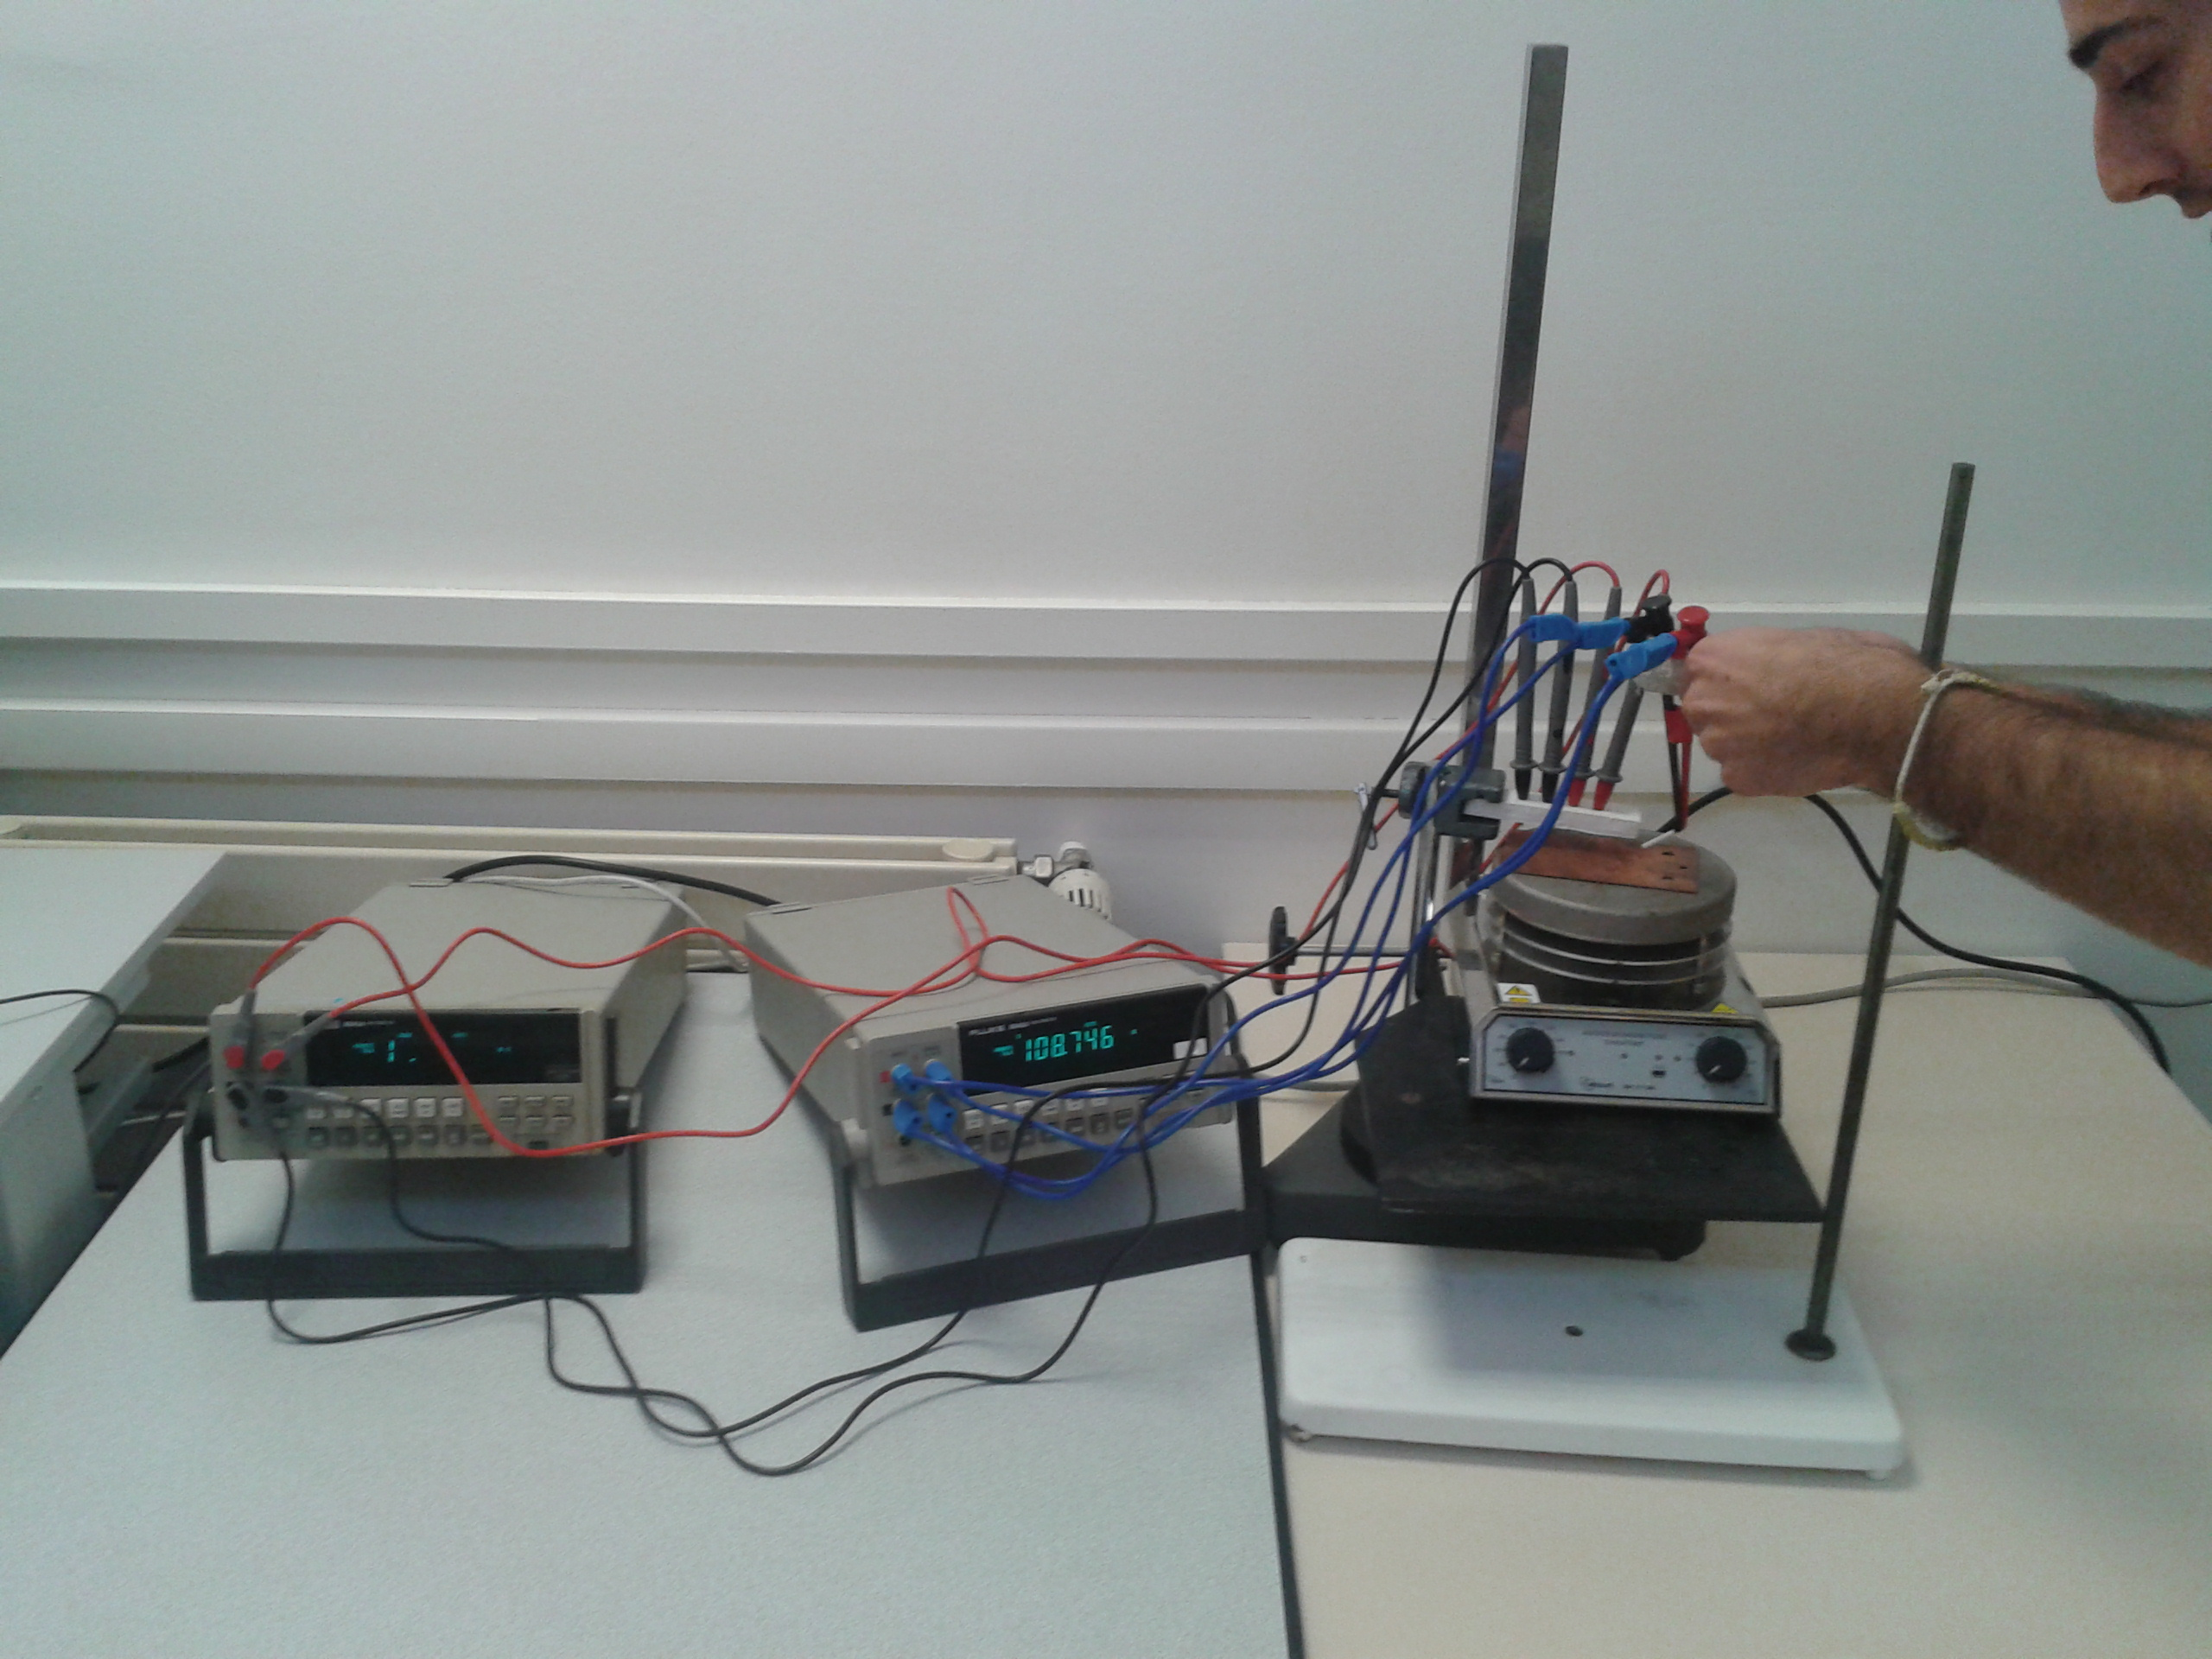
\includegraphics[width=9cm]{./images/photo1.jpg}
		\caption{Montage général}
		\label{photo1}
	\end{center}
\end{figure}

\newpage

\begin{figure}[!t]
  \begin{center}
		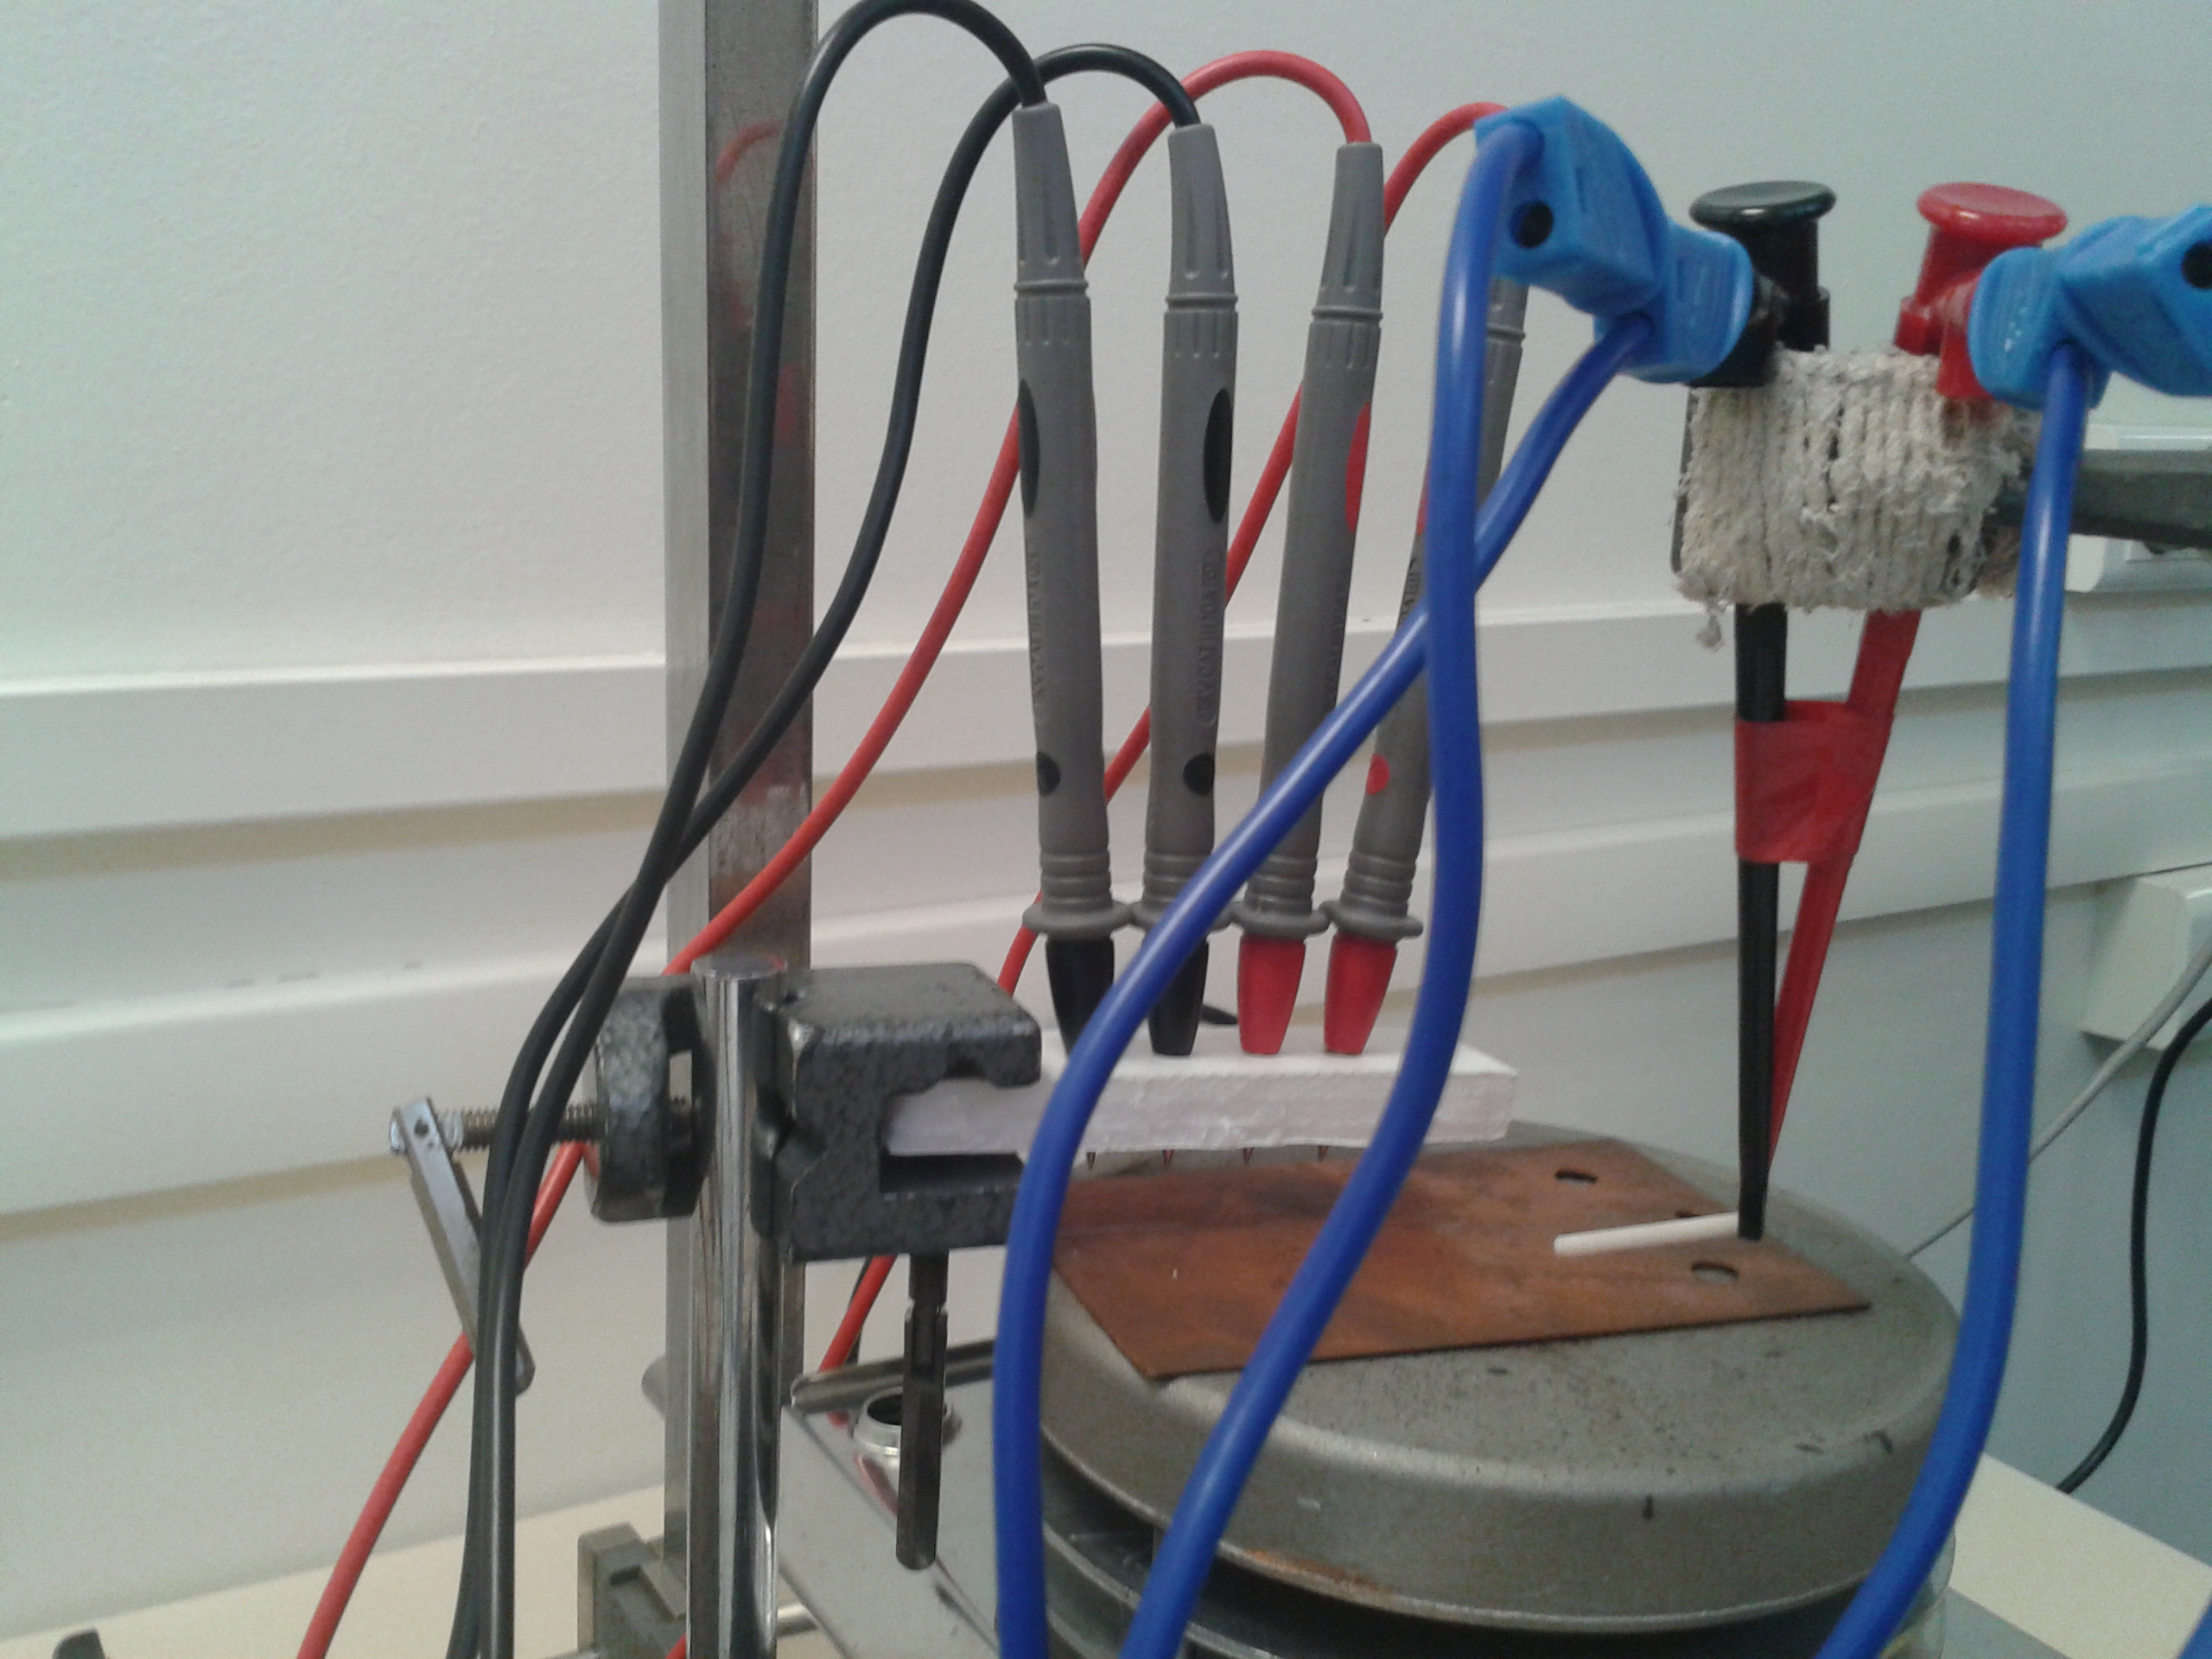
\includegraphics[width=9cm]{./images/photo2.jpg}
		\caption{Gros plan sur les sondes de mesure de résistance et de température}
		\label{photo2}
	\end{center}
\end{figure}
\begin{figure}[h]
  \begin{center}
		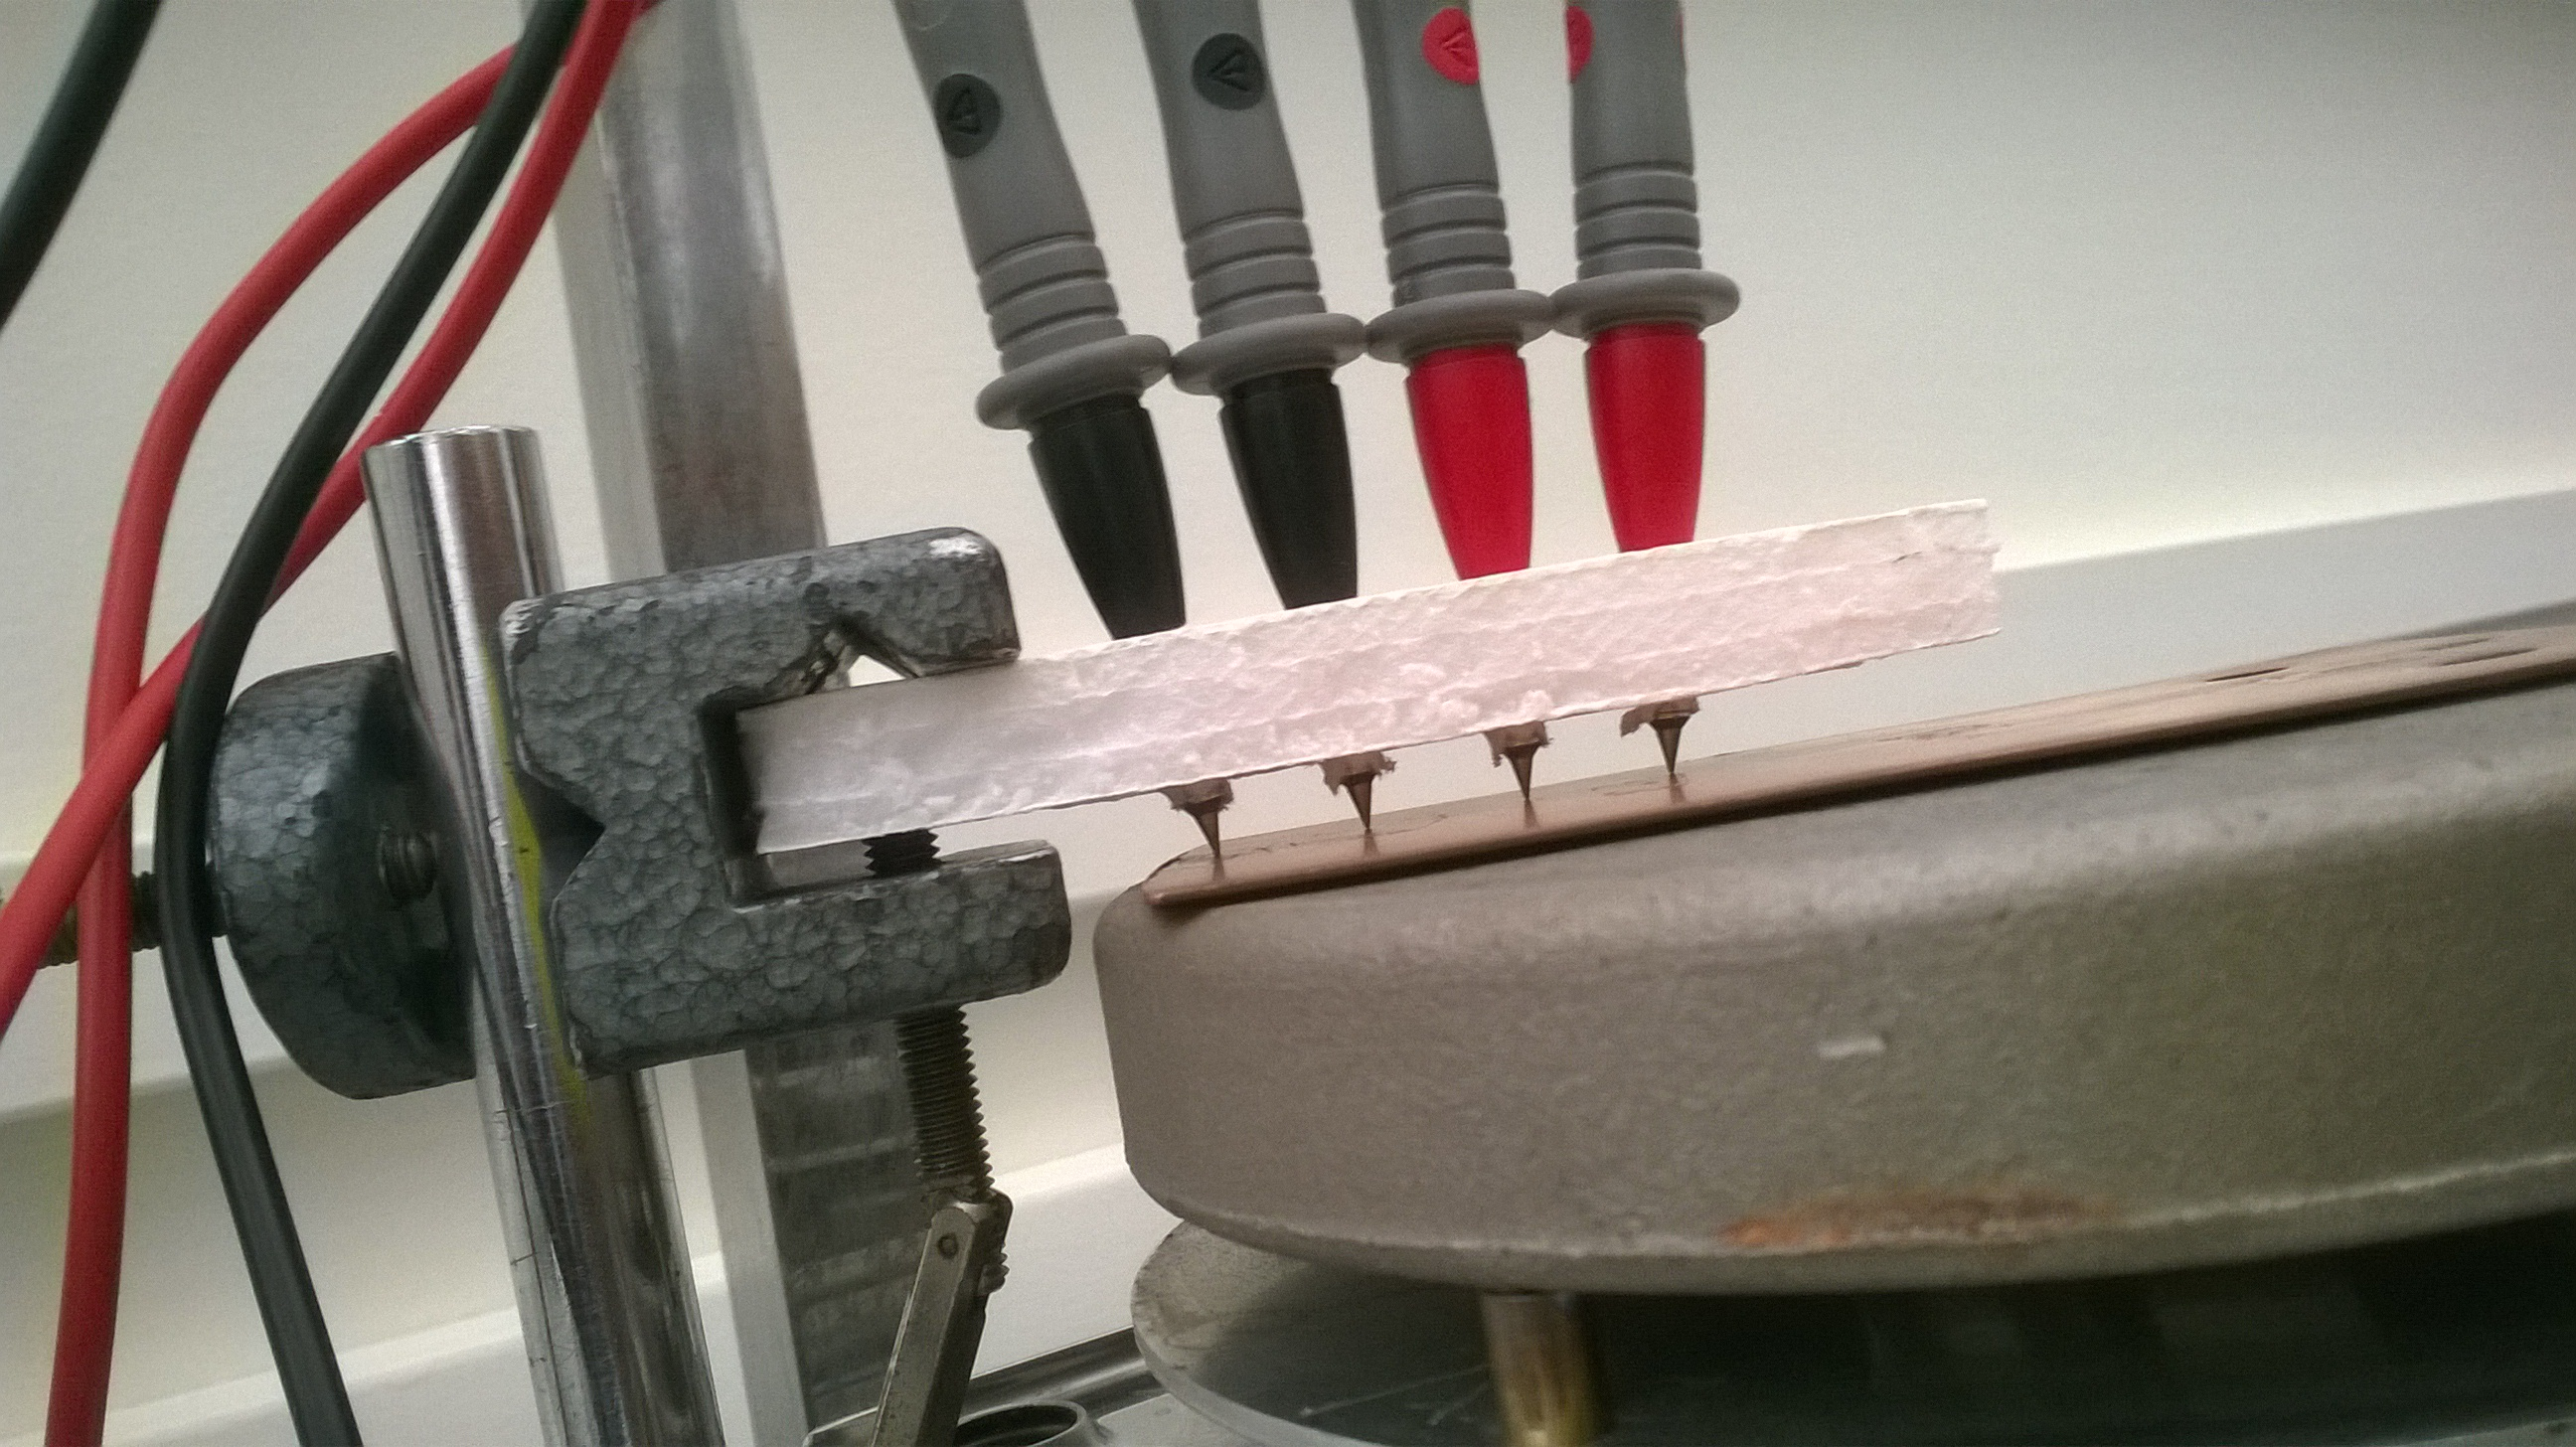
\includegraphics[width=9cm]{./images/photo3.jpg}
		\caption{Les 4 pointes en contact}
		\label{photo3}
	\end{center}
\end{figure}

Sur les 2 photos suivantes : Figures \ref{photo4} et \ref{photo5}, on peut voir le porte-échantillon rempli de billes de verre, et dans lequel est inséré la sonde de température, ce montage étant utilisé dans le cas du refroidissement à l'azote liquide (on verse l'azote dans ce porte-échantillon adapté à ce type de manipulations à très basse température.

\newpage

\begin{figure}[!t]
  \begin{center}
		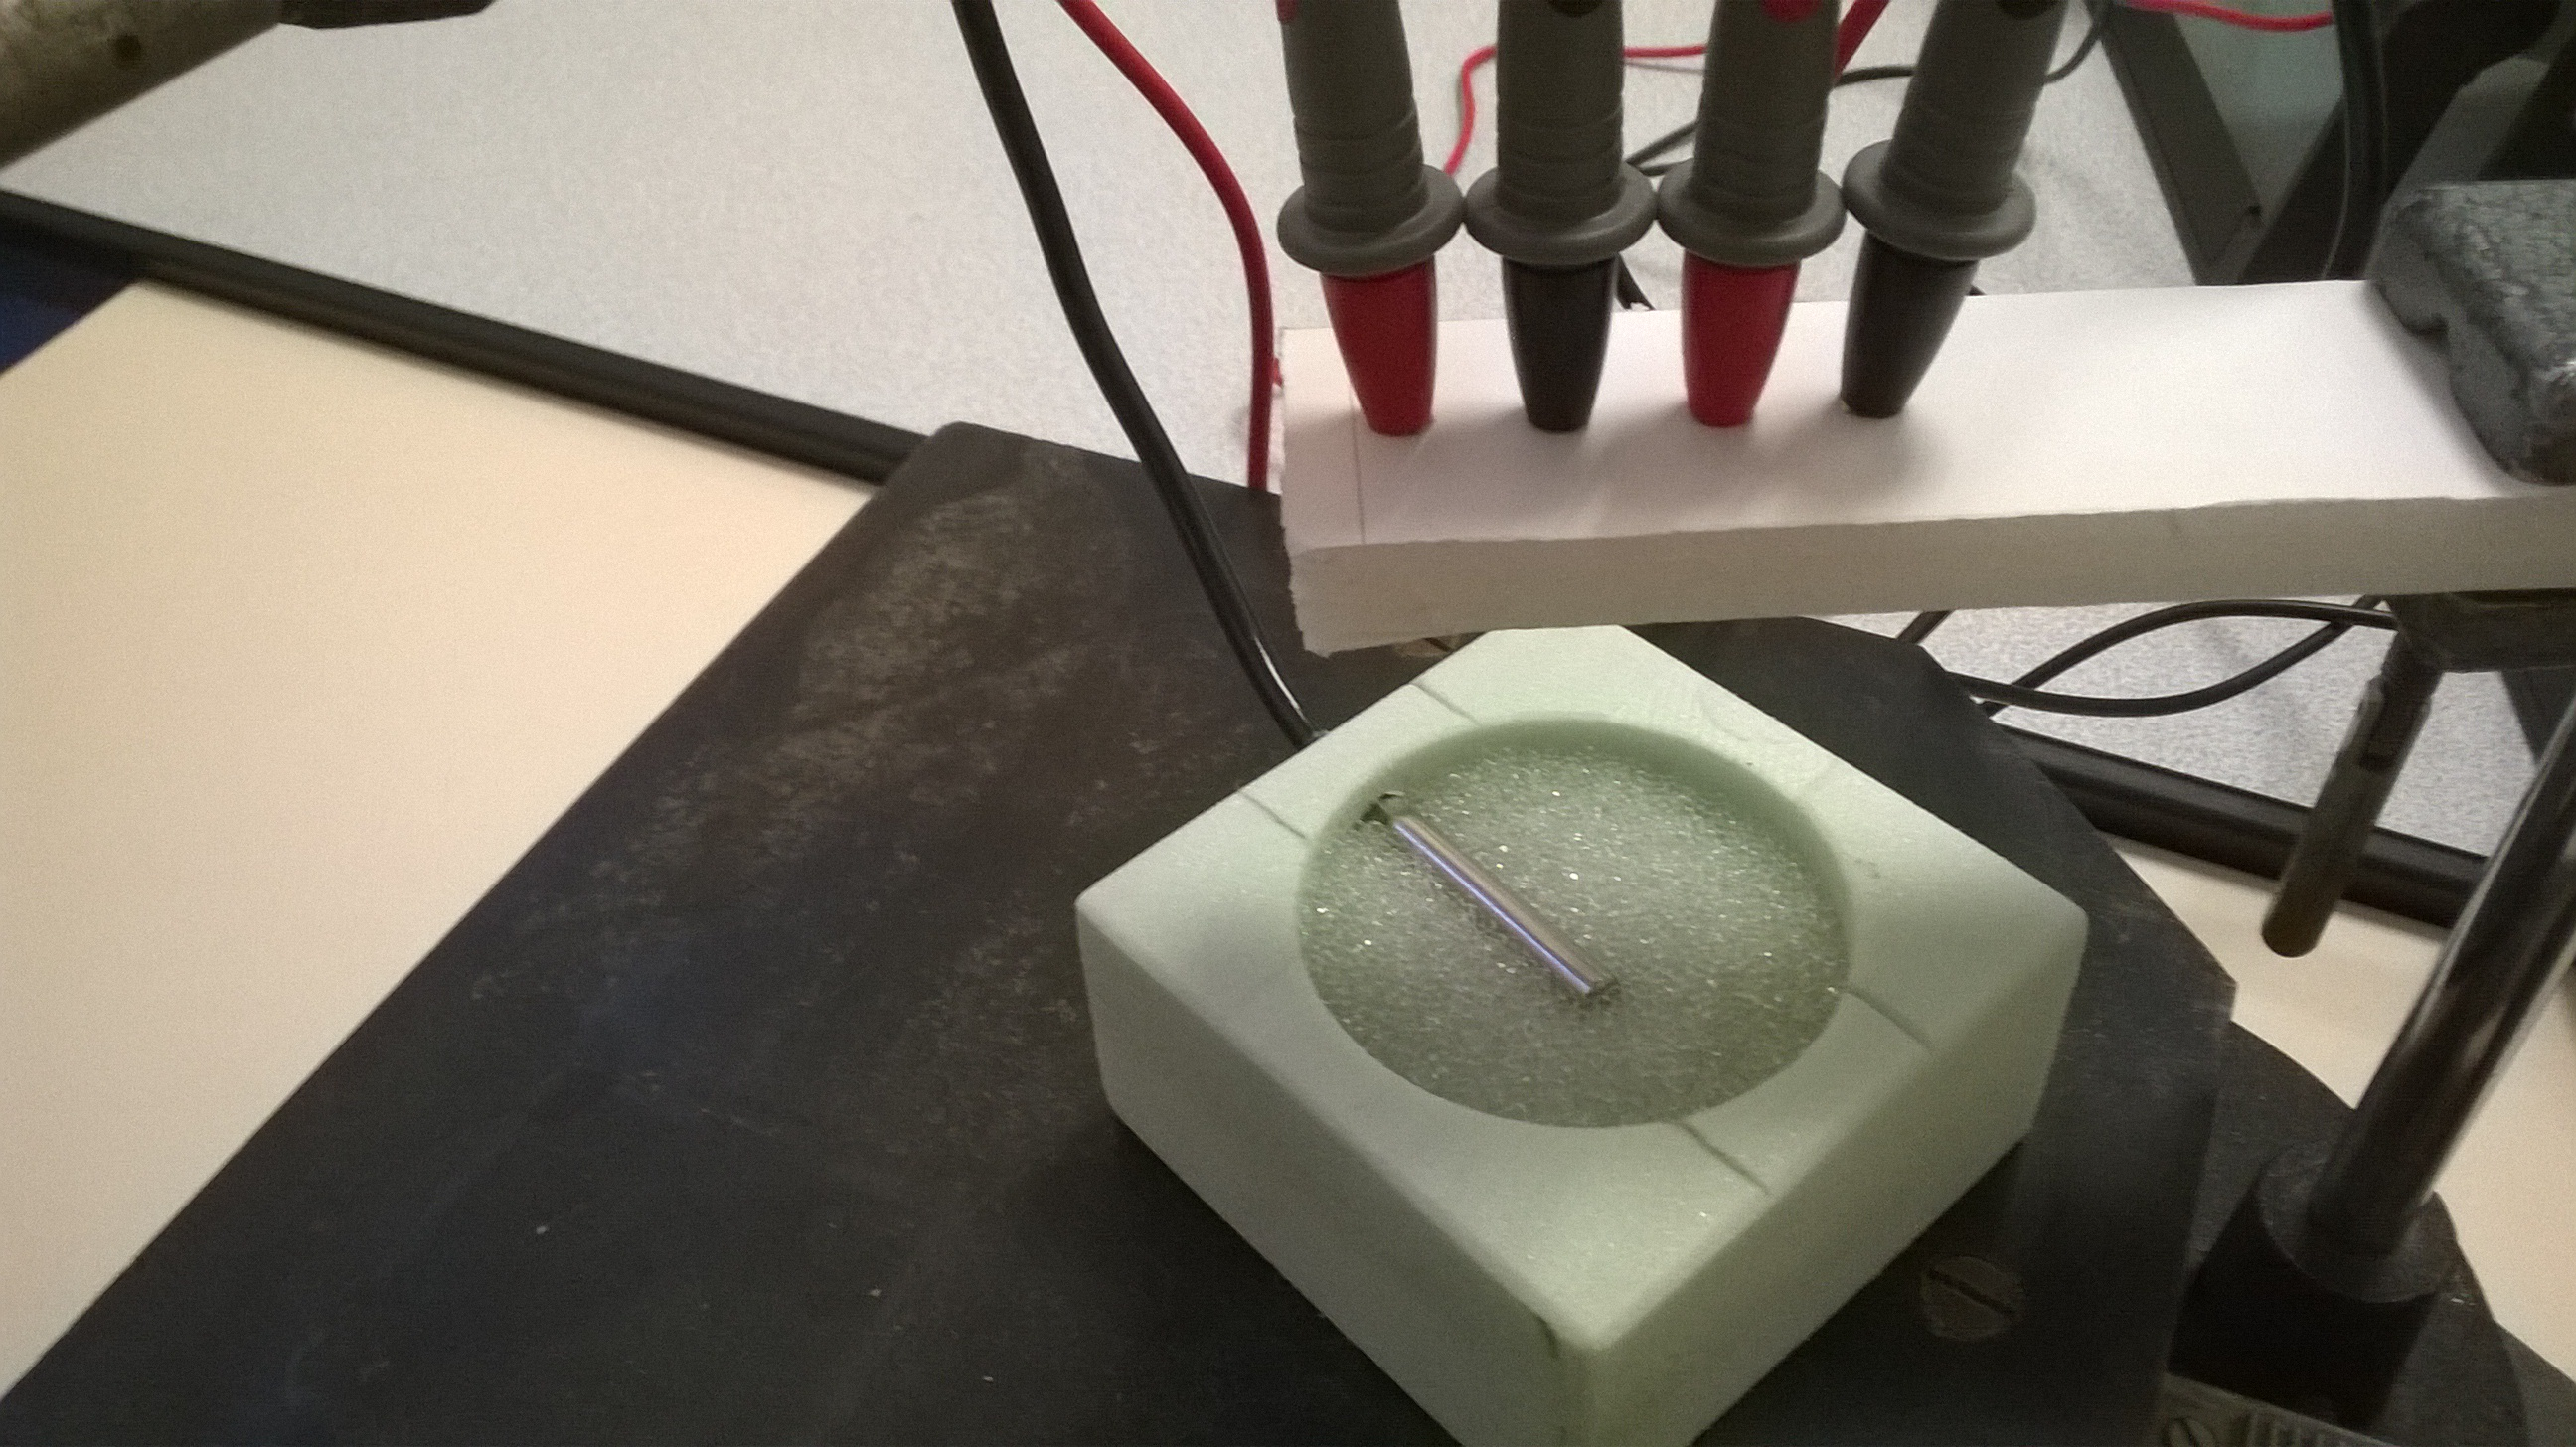
\includegraphics[width=7cm]{./images/photo4.jpg}
		\caption{Porte-échantillon pour le refroidissement à l'azote liquide}
		\label{photo4}
	\end{center}
\end{figure}

\begin{figure}
  \begin{center}
		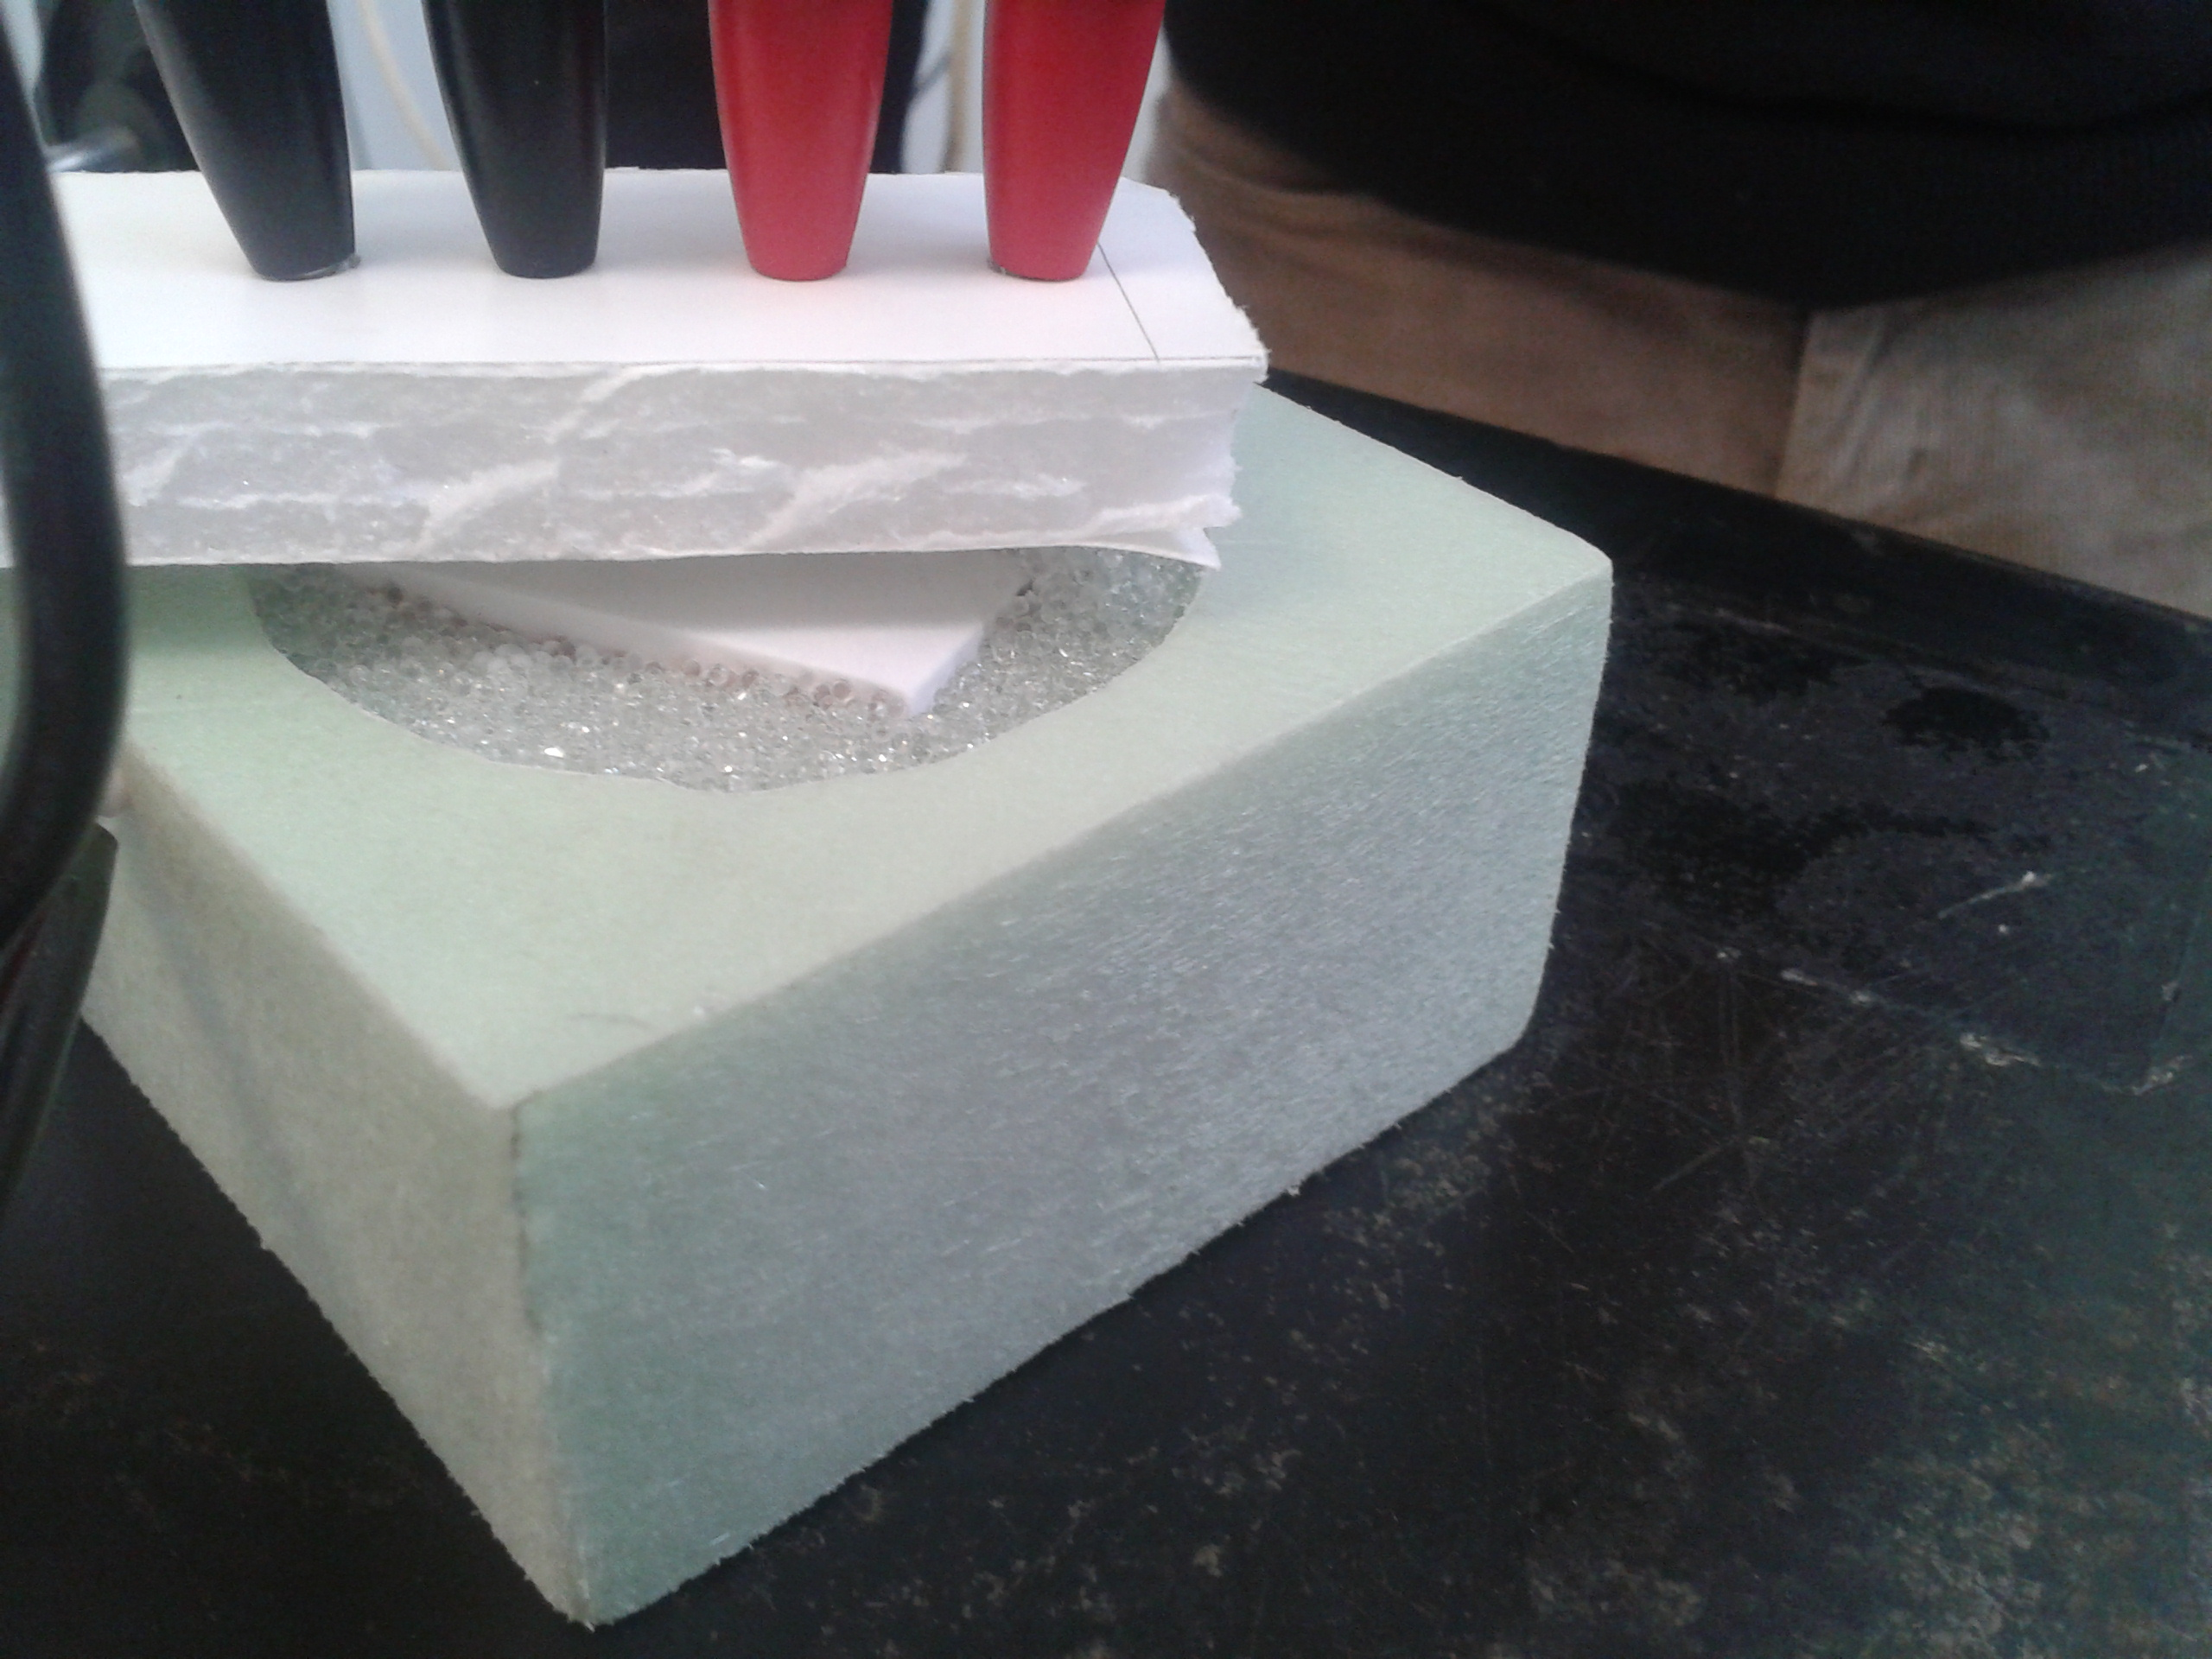
\includegraphics[width=7cm]{./images/photo5.jpg}
		\caption{Les 4 pointes en contact au cours d'une mesure avec refroidissement à l'azote liquide}
		\label{photo5}
	\end{center}
\end{figure}

Voici enfin une photo du montage à effet Hall [Figure \ref{photo_hall}], que nous avions commencé à préparé, 
mais que nous n'avons malheureusement pas eu le temps de terminer. Nous voulions utiliser un électroaimant, 
on peut aussi observer une source de courant sur la table. %ainsi qu'un porte-échantillon à gauche de l'aimant.

\begin{figure}[!t]
  \begin{center}
		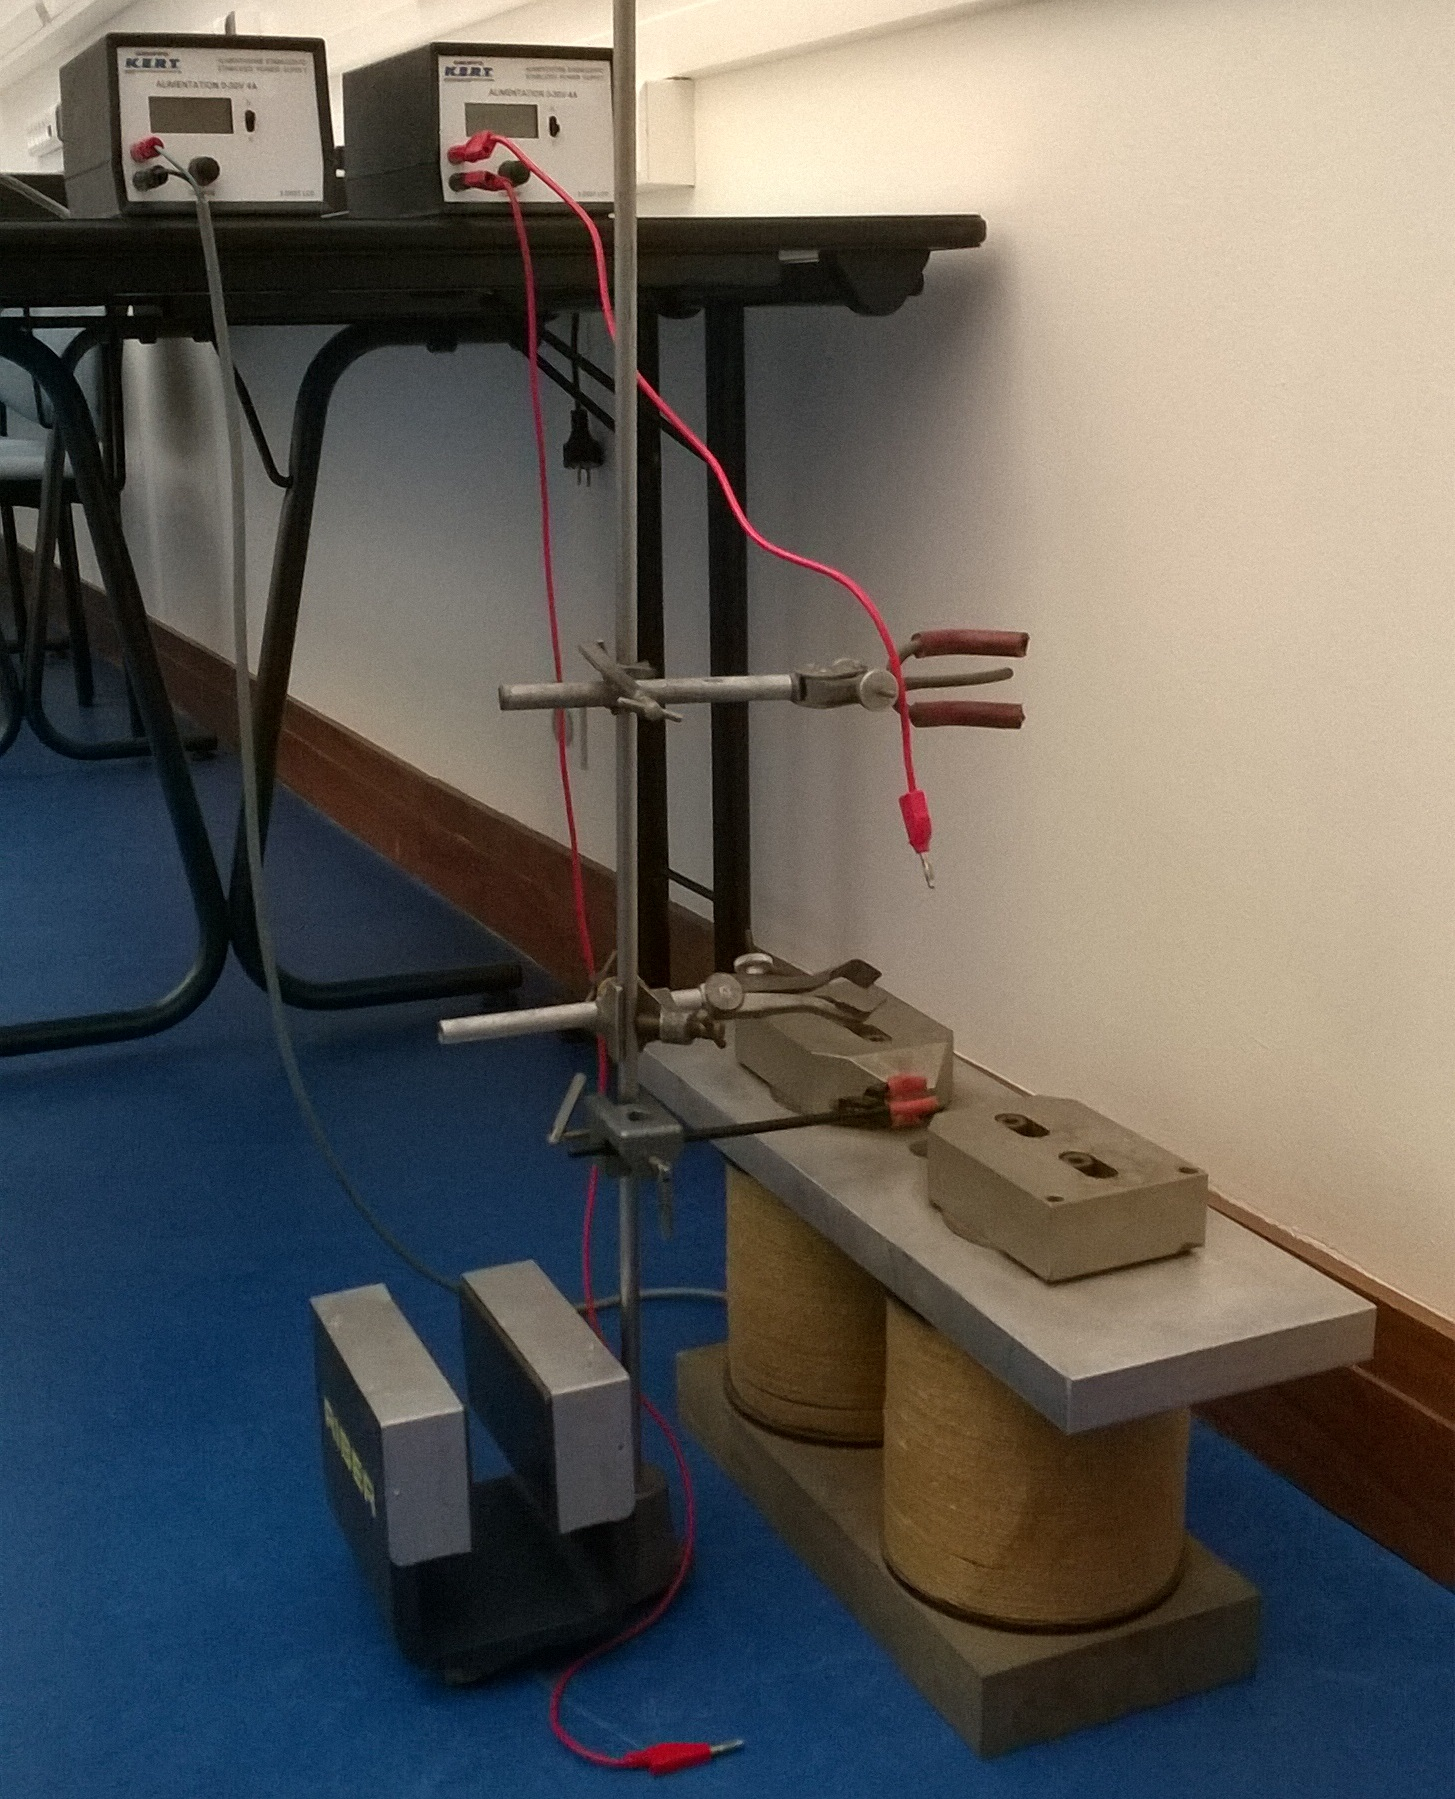
\includegraphics[height=6cm]{./images/photo_hall.jpg}
		\caption{Montage pour la mesure à effet Hall}
		\label{photo_hall}
	\end{center}
\end{figure}

\newpage

\subsection{Conditions expérimentales}
Nous avons utilisé Labview pour réaliser les acquisitions des deux résistances mesurées.
Nous avons simplement posé la plaque de cuivre sur une plaque chauffante et mesuré sa résistance en fonction de la température en 4 pointes, entre 25\celsius{} et 205\celsius{}.


Pour le silicium, nous voulions détecter un palier de conductivité (car il s'agissait d'échantillons dopés), et nous savions que ce palier risquait de se trouver à une température inférieure ou égale à la température ambiante.
Donc, pour pouvoir étudier ce palier, nous avons dû baisser fortement la température et nous avons utilisé de l'azote liquide pour cela.
Nous avons également placé des billes de verre dans notre porte-échantillon pour augmenter l'inertie thermique du montage et nous permettre d'avoir une montée en température relativement lente.
La sonde de température a été insérée dans le porte-échantillon par un trou percé sur le côté (voir Figure \ref{photo4}). De cette façon, elle peut être en contact du silicium et être entourée par les billes de verre.
De ce fait, elle mesure bien mieux la température du silicium que si on l'avait simplement posée sur l'échantillon.


\paragraph{Pourquoi une mesure 4 pointes (et pas tout simplement 2) ?}
La mesure 4 pointes consiste à injecter un courant avec deux pointes et à mesurer une tension avec deux autres placées entre les deux premières.
Cette méthode permet de s'affranchir des résistances des fils et des résistances de contact.
Elle est donc particulièrement utile pour mesurer des résistances de l'ordre de l'$\Omega$ ou inférieures, car c'est l'ordre de grandeur des résistances parasites.
Par contre, elle est peu utile pour les hautes résistances (plusieurs k$\Omega$, M$\Omega$), donc nous aurions mesuré en 2 pointes pour un isolant par exemple.


\paragraph{Principe et étalonnage de la sonde}
Nous avons étalonné la sonde Pt en deux étapes :

\begin{itemize}
  \item en la plaçant dans de l'eau que nous avons fait bouillir, nous avons pu mesurer la résistance de la sonde à une température de 100\celsius{}.
  \item en la plaçant ensuite dans de l'eau pleine de glaçons, nous avons fait la même chose pour 0\celsius{}.
\end{itemize}

La résistance du platine augmente très linéairement avec la température, c'est une propriété de ce matériau.
On obtient alors la caratéristique R(T) : en mesurant la résistance du Platine, on peut en déduire sa température (donc idéalement la température de l'échantillon).


\paragraph{Interfaçage grâce à Labview}
L'utilisation de l'outil informatique pour mener à bien l'expérience était prévu pour cet AE 
et en constituait une des principales caractéristiques. En effet notre encadrant nous avait fortement recommandé 
d'automatiser les mesures pour faciliter la prise de données tout en gagnant en savoir-faire expérimental. L'outil de 
prédilection pour ce type de mesure est le logiciel \emph{LabVIEW} qui permet de réaliser l'acquisition et le traitement des données. 
Nous avons donc décidé d'utiliser ce logiciel. Le but était de pouvoir contrôler les deux multimètres avec l'ordinateur. 
La prise de données par voie informatique comporte trois volets que nous avons dû nous approprier successivement : 

\begin{enumerate}
\item la connexion des appareils à l'ordinateur ; 
\item leur reconnaissance par ce dernier ; 
\item et le codage du code LabView. 
\end{enumerate}

La première étape a été réalisée grâce à deux câbles \emph{smart488}, mais le laboratoire n'ayant qu'un seul câble de ce type, nous avons dû en commander en deuxième.
Ces câbles permettent le passage d'une sortie GPIB à une sortie USB et possèdent un contrôleur intégré. 
C'est ce contrôleur qu'il a fallu régler, grâce à un logiciel dédié, pour pouvoir détecter les deux multimètres 
via l'ordinateur. Nous avons aussi utilisé le logiciel NI-Max pour vérifier la compatibilité de ces éléments avec Labview. 
Après cela nous avons entamé l'étape d'écriture du code graphique Labview [Figure \ref{code_labview}]. Ce code devait nous permettre d'acquérir 
simultanément, et dans le temps, les signaux des deux multimètres, qui correspondent à la température de la sonde 
et à la résistance de l'échantillon. L'acquisition se fait pendant un laps de temps prédéfini. Les résultats obtenus sont présentés sous forme de tableau de nombres dans un fichier texte qui peut être lisible par un logiciel comme gnuplot ou Excel.
Nous avons en effet utilisé gnuplot par la suite pour tracer nos courbes.

\begin{figure}[!t]
  \begin{center}
		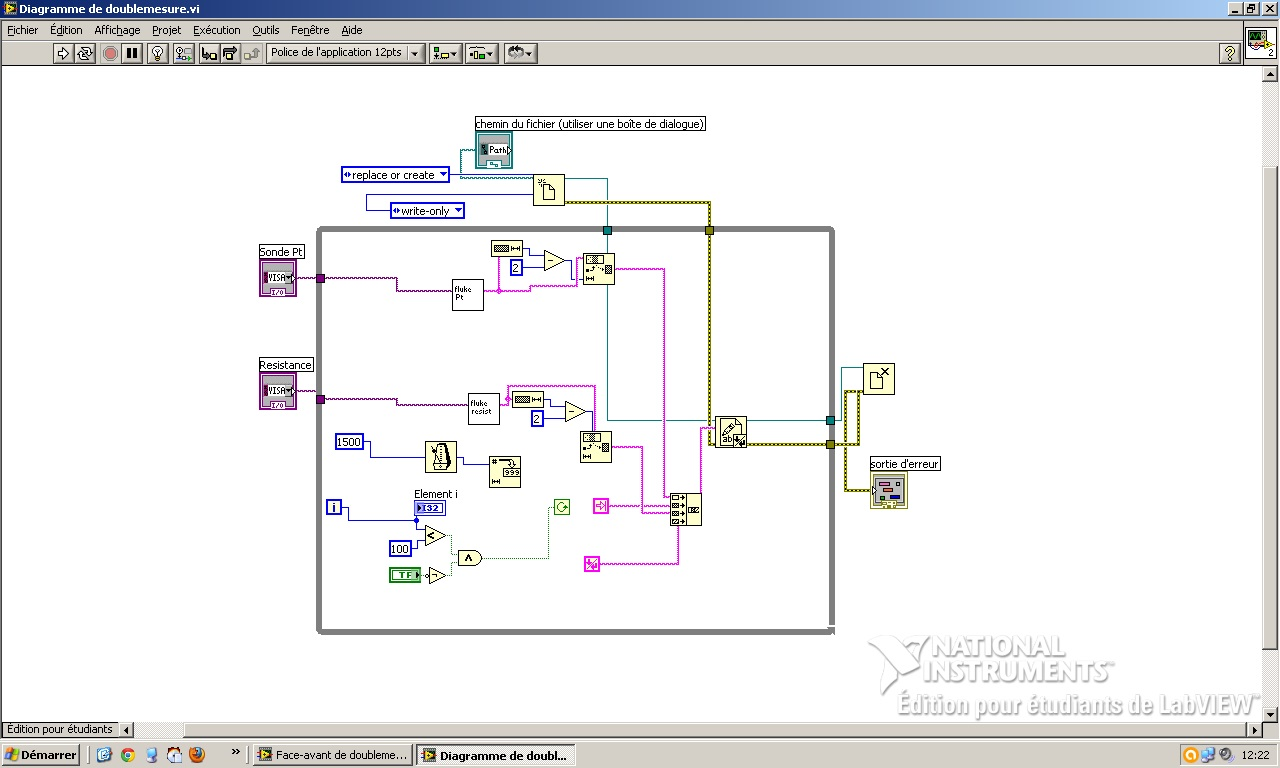
\includegraphics[height=6cm]{./images/labview.jpg}
		\caption{Code de notre programme Labview}
		\label{code_labview}
	\end{center}
\end{figure}


\subsection{Difficultés expérimentales}
Deux principales difficultés expérimentales se sont posées lors de cette activité expérimentale.
Tout d'abord il y a eu le problème de l'automatisation des résultats et de l'interfaçage avec l'ordinateur.
Nous avons eu du mal à réaliser chacune des trois étapes liées à l'automatisation des mesures, mais plus particulièrement 
pour la détection des instruments par l'ordinateur, ceci mettant en jeu différents composants tels que le 
multimètre, le câble smart488 et Labview.

D'autre part le contact entre les électrodes et l'échantillon s'avéra bien plus délicat que prévu. 
En effet l'utilisation du montage à quatre pointes oblige à avoir quatre contacts stables.
Nous avons d'abord utilisé de la laque d'argent pour réaliser les contacts, mais cela ne s'est pas avéré facile à mettre en place ni très efficace.
Nous avons donc implémenté le montage tel qu'il apparaît dans les photos [Figures \ref{photo1} à \ref{photo5}]. Le premier essai sur le cuivre donna des résultats 
très cohérents mais les essais sur les échantillons de silicium donnaient des valeurs très instables. 
En effet la valeur de la résistance changeait de plusieurs ordres de grandeurs selon la pression exercée sur les 
pointes. On soupçonne les fils et les pointes d'être a l'origine de ces fluctuations (contacts imparfaits), mais une piste intéressante est l'hétérogénéité de la surface de l'échantillon de silicium. 
En effet le silicium au contact de l'air s'oxyde et on obtient une couche de SiO2 à la surface de l'échantillon. 
La variation de la résistance selon la pression exercée sur les pointes peut donc provenir du fait que la pointe 
traverse où pas cette couche. Cependant lorsque on exerce une pression constante on obtient des résultats cohérents avec la nature semiconductrice du silicium comme on pourra le voir dans nos résultats. Une façon d'obtenir cette pression constante et donc un meilleur contact est d'utiliser des pointes à ressorts, fixées solidement au support. Cependant nous n'avons pas pu nous procurer de tels contacts avant la fin de l'activité et nous avons du réaliser plusieurs fois la même expérience jusqu'à obtenir une mesure stable.

\subsection{Résultats}
Pour le cuivre, nous avons simplement observé que la conductivité diminue quand on augmente la température (voir courbe).
[donner un ordre de grandeur de la conductivité du cuivre sur cette plage de température si elle est bonne]


Pour le silicium, nous avons observé une conductivité croissante avec la température, ce qui est cohérent. Nous avons aussi observé un palier aux alentours de [20\celsius{}; 80\celsius{}], ce qui semble cohérent aussi.
À haute température, on observe à nouveau une croissance de la conductivité, 
puis les contacts se sont dégradés donc on n'a pas pu monter plus haut en température.

\subsubsection{Courbes}


\subsection{Discussion des résultats}

L'endroit où se trouve le palier paraît cohérent, pour le Si il est autour de la température ambiante (cf. \cite{kittel_introduction_1976}), 
c'est pourquoi le Si est utilisé dans l'électronique.


\subsection{Conclusions}

